\chapter{Implementation}
\label{implementation}
Machine Learning and especially Deep Learning systems are resource intensive algorithms that need large amounts of both training data and computation time. Because the computations made in ML typically is large matrix operations, it is preferable to run most of the training on GPUs. This has coloured some of the implementation choices.

This chapter contains a description of the software used to implement the ML structures and search algorithms used in the experiments in chapter \ref{exp1}, \ref{exp2}, and \ref{exp3}.

\section{Python}
Python as a programming language choice for Machine Learning is becoming more and more common. While Python out-of-the-box is not suited for the type of operations necessary for ML due to its slow run time, a number of excellent packages for Machine Learning and data-processing provide a workaround of Pythons native limitations. The language also provides a rapid prototyping environment, as well as a large community which makes troubleshooting easier. 

\subsection{TensorFlow}
TensorFlow\cite{tensorflow} is an open source symbolic math library. It is commonly used for Machine Learning and neural network implementation as it makes it possible to design graph structures in Python. The graphs created operate on n-dimensional matrices called tensors through graphs of mathematical operations and is executed with low-level backend libraries such as \textit{C} or \textit{Fortran}.

TensorFlow also provides support for different computing devices, meaning a CPU implementation can be made to run on GPU with excellent benefits to computation time. The implementation used in this thesis runs all weight optimization on the GPU, but as there is a substantial amount of computation performed on the CPU between each round of model training, the benefit of training on the GPU is not as great as it could be. Future implementations could take advantage of customized graph-nodes to perform tournament searches quicker. 

\subsection{Keras}
Keras\cite{keras} is a high-level Machine Learning API that has a generalized and modular approach to neural network implementation. It depends on a specialized, well-optimized low-level backend library to perform its necessary tensor operations, and supports the use of TensorFlow, Theano or CNTK backend for that purpose. Keras provides superior debugging feedback to a stand-alone TensorFlow implementation, while it still supports micro-managing of parameters through tensors or matrices, making Keras simple to implement while allowing for a high level of model customization.

\subsection{Other packages}
Other packages used to implement the experiments and analyzation of their results:
\begin{itemize}
    \item SciPy: Providing a package containing statistical tests such as the Mann-Whitney-Wilcoxon U-test.
    \item Pickle: Used during experimentation to store results for later visualization and analysis.
    \item Matplotlib: Used for the visualization of experiment results.
    \item Numpy: Used for most mathematical operations not available through native Python functions 
    \item GraphViz: Used for generating graphs of PathNet structures for debugging. Multiple paths are drawn in the same graph with training amount in each module.
    \item Reprint: Used to manage search terminal output by refreshing multi-line output in the terminal, simplifying search debugging.
\end{itemize}

\section{PathNet implementation}
As the same code was used in all experiments in this thesis, it was designed to be highly modular and easily configurable. This object-oriented design is based around Keras's already generalized approach to Machine Learning.

\subsection{Code structure}
Modules are implemented through Layer-objects of two types: Dense-layers to hold fully-connected modules and Conv-layers to hold convolutional modules. Each module type is defined by a configuration-dictionary describing the smaller NN's that constitute a module: 

\begin{lstlisting}[language=Python]
    dense = [{'out': 20, 'activation': 'relu'}, 
             {'out': 5, 'activation': 'softmax'}]
    conv  = [{'channels': 10, 'kernel': (3,3), 
              'stride': (1,1), 'activation':'relu'}]
\end{lstlisting}
In the example above, the two lists of configuration-dictionaries yield different module-types. The "\emph{dense}"-list defines a module with a fully connected NN with two hidden layers, where the first layer have 20 nodes with ReLU-activation and the second use a softmax-activation. The "\emph{conv}"-list defines a one layer CNN where the two-dimensional convolution have 10 channels, use a three-by-three kernel with a stride\footnote{As mentioned in section \ref{background:ML}, stride is how far the kernel moves in each dimension between each matrix multiplication.} of 1 in each dimension and a ReLU-activation.

The Layer-objects also define other operations that can be added as needed on object-instantiation. These are:
\begin{itemize}
    \item \emph{BatchNormalization}\cite{batchnorm} (in Conv-modules). This operation normalizes the output from a layer within each training-batch. This is to average potential extremes/outliers in layer outputs to limit radical gradients during training.
    \item \emph{MaxPooling} (after the last Conv-layer). The operation reduces the dimensionality of a layer output by reducing each x-by-y\footnote{Here, only MaxPooling of 2-by-2 windows are performed. This means a 10-by-10 feature map would be reduced to 5-by-5, where each value is the maximum of each neighboring pixel in the original feature map.} window of pixels to the max value within that window. \emph{Pooling} is normally used to limit the number of features, usually for computational reasons, or to reduce the possibility of overfitting.
    \item \emph{Flatten} (before the first Dense-layer). This \textit{"housekeeping"} functionality takes some n-dimensional tensor input and flattens it to a vector to be input into the fully connected NN in a Dense-layer.  
\end{itemize}

As mentioned in section \ref{background:pn}, each task has its unique task-specific final layer that defines the output from PathNet for that task. This concluding layer is defined by Task-objects which contain one layer of fully connected nodes, an activation function, and an output-size specific to that task. Only classification-tasks are performed in this thesis, so all tasks use a softmax-activation. The Task-object also contain some meta-info about the model they are a part of, such as input-dimensions, optimizer used for this task, a learning-rate, and loss-function. 

The PathNet-object is the only one utilizing the Layer and Task-objects. Through hard-coded static methods, a PathNet structure is created for each experimental run. The methods randomly initialize all layers, modules, and configurations needed to start training. The PathNet-object also contains functionality for generating random paths and Keras-models from a given path-description and Task-object. It also includes a training-counter for each module and an interface for updating this value. Lastly, there is some \textit{housekeeping} functionality such as saving and locking modules, and a TensorFlow-session backend reset (see section \ref{implementation:problems}).

\section{Search implementation}
\label{implementation.search}
As with PathNet, the tournament-search has a modular implementation for easy adaptability and reuse in all experiments. Based on a hyperparameter-dictionary, the search method uses predetermined functions for different GA operations, such as selection-schemes for winner selection or path mutation. The selection-schemes used is winner-replace-all, where a mutation of the winner replace all other genomes in the tournament, and a 3-to-2 scheme where the two winners of a tournament of size 3 are combined with a crossover-algorithm and the offspring replace the tournaments looser.

Every generation, a Reprint-structure is updated, which gives a terminal output of the search progress (see figure \ref{fig:searchoutput} for a screen capture of an experimental run).
\begin{figure}[ht]
    \centering
    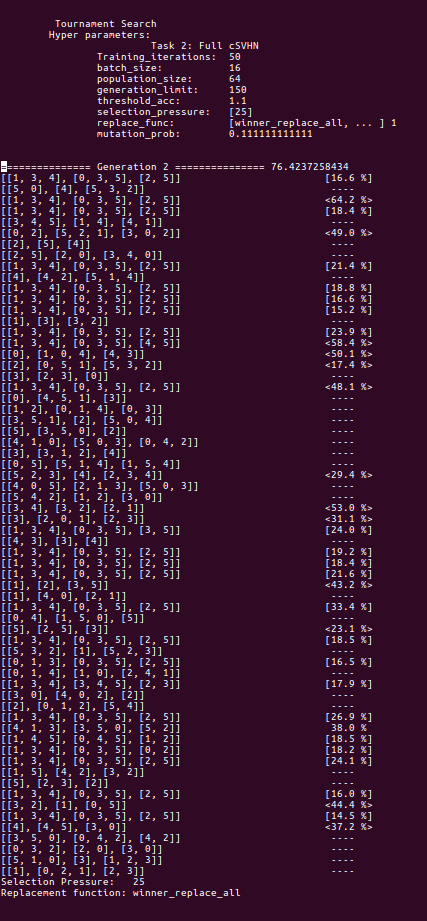
\includegraphics[width=0.6\textwidth]{Chapters/3.Implementation/figures/search_output.png}
    \caption[Terminal search output]{Screencapture of terminal output during a search. The top section contains hyperparameters for this search as well as the current generation number. Underneath, the current population-state can be seen, as well as some accuracies in the right margin. For these, \big[ \big] means the accuracy is outdated by training, \big< \big> means the value within is a training accuracy, .... means the path is not evaluated yet, and a plain percentage is the actual fitness of that path. At the bottom, the current generations selection pressure is printed, as well as the selection scheme.}
    \label{fig:searchoutput}
\end{figure}

\section{Notable implementation differences}
\begin{itemize}
    \item Implementation is built upon the Keras API and is more modular with its object-oriented structure
    \item Path-fitness is not the negative error, but classification accuracy. 
    \item For the selection pressure experiments in chapter \ref{exp2} and \ref{exp3}, the fitness calculation is performed in a separate evaluation step after training. See \ref{exp2:implementation} for details and reasoning.
\end{itemize}

\section{Implementation difficulties} 
\label{implementation:problems}
Some implementation difficulties occurred during the work on this thesis. Most of these were due to ignorance of certain TensorFlow effects. Some of the most noteworthy are listed here to help with implementations in the future.
\begin{itemize}
    \item The TensorFlow backend session is not made for creating multiple graphs, and memory leaks occur if the session for training multiple models. Functionality in TensorFlow makes it possible to reset a TensorFlow session, but all graph-variables has to be reinitialized afterward. 
    \item TensorFlow's default is to use all available GPU-memory. Setting the TensorFlow-sessions GPU-options "allow-growth" parameter to 4 sets memory allocation to be done as needed.
    \item Memory allocated by a TensorFlow session is not freed when the session ends, but when the Python process that initialized it is ended.
\end{itemize}

\section{Datasets}
\subsection{MNIST}\label{Implementation:MNIST}
One of the most commonly used datasets for testing image classifiers is the MNIST\cite{MNIST} set of hand-drawn digits. These 28-by-28 images each contain a digit from 0 through 9. The 60 000 labeled images are distributed about evenly across all ten classes. 

\begin{figure}[p!]
    \centering
    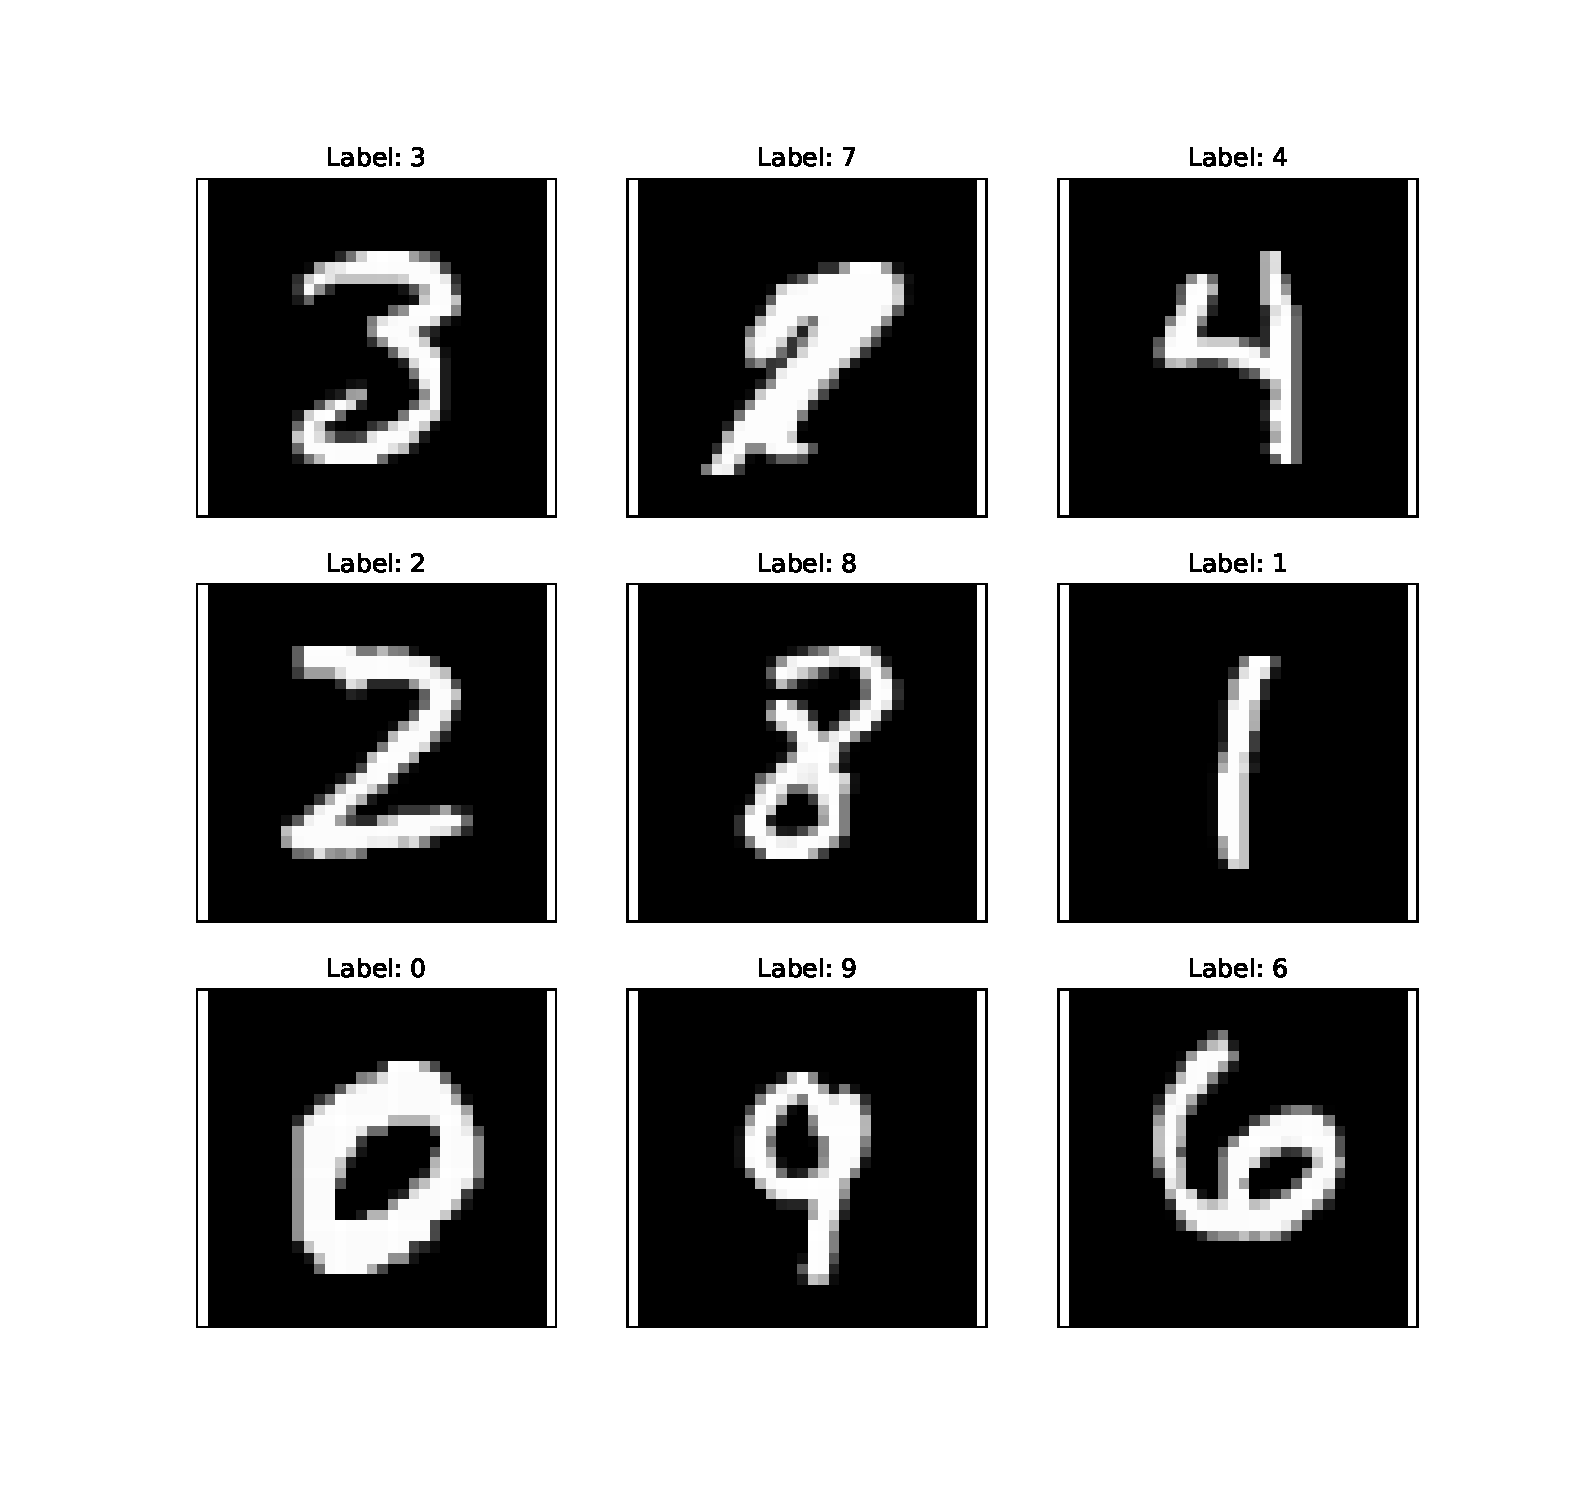
\includegraphics[width=0.8\textwidth]{Chapters/3.Implementation/figures/MNIST.pdf}
    \caption[MNIST example]{Nine images from the MNIST dataset.}
    \label{fig:mnist}
\end{figure}

MNIST is a simple dataset as far as image classification goes (see section \ref{exp1:BIN.results}). The small grayscale images contain only one small object in the middle of the image, and almost all pixels is either 0 (background) or 1 as seen in figure \ref{fig:mnist}. This makes the classification task rather easy. A list of reached accuracies\footnote{As of March 2018} can be found on the dataset's web page\cite{mnistpage} where the lowest error rate is 0.23\cite{goodmnist}, and a KNN-classifier without preprocessing is claimed that to achieve a validation accuracy of 97.17. 


\subsection{SVHN}\label{Implementation:SVHN}
The Street View House Number\cite{SVHN} dataset is real-world images from Google Street View made for machine learning development. The original dataset contains over 600 000 variable resolution images of house numbers and bounding boxes around each digit with a label for each box. In this thesis, the version of SVHN used is made of cropped images (cSVHN) as seen in figure \ref{fig:csvhn}. These images are 32-by-32 colored images that are made to function in somewhat the same way MNIST does, with a simple object and static size. Note, however, that where MNIST images contain only the object that is the basis for classification, cSVHN contain distractions (noise) in the image such as half-cropped neighboring digits. 

\begin{figure}[p!]
    \centering
    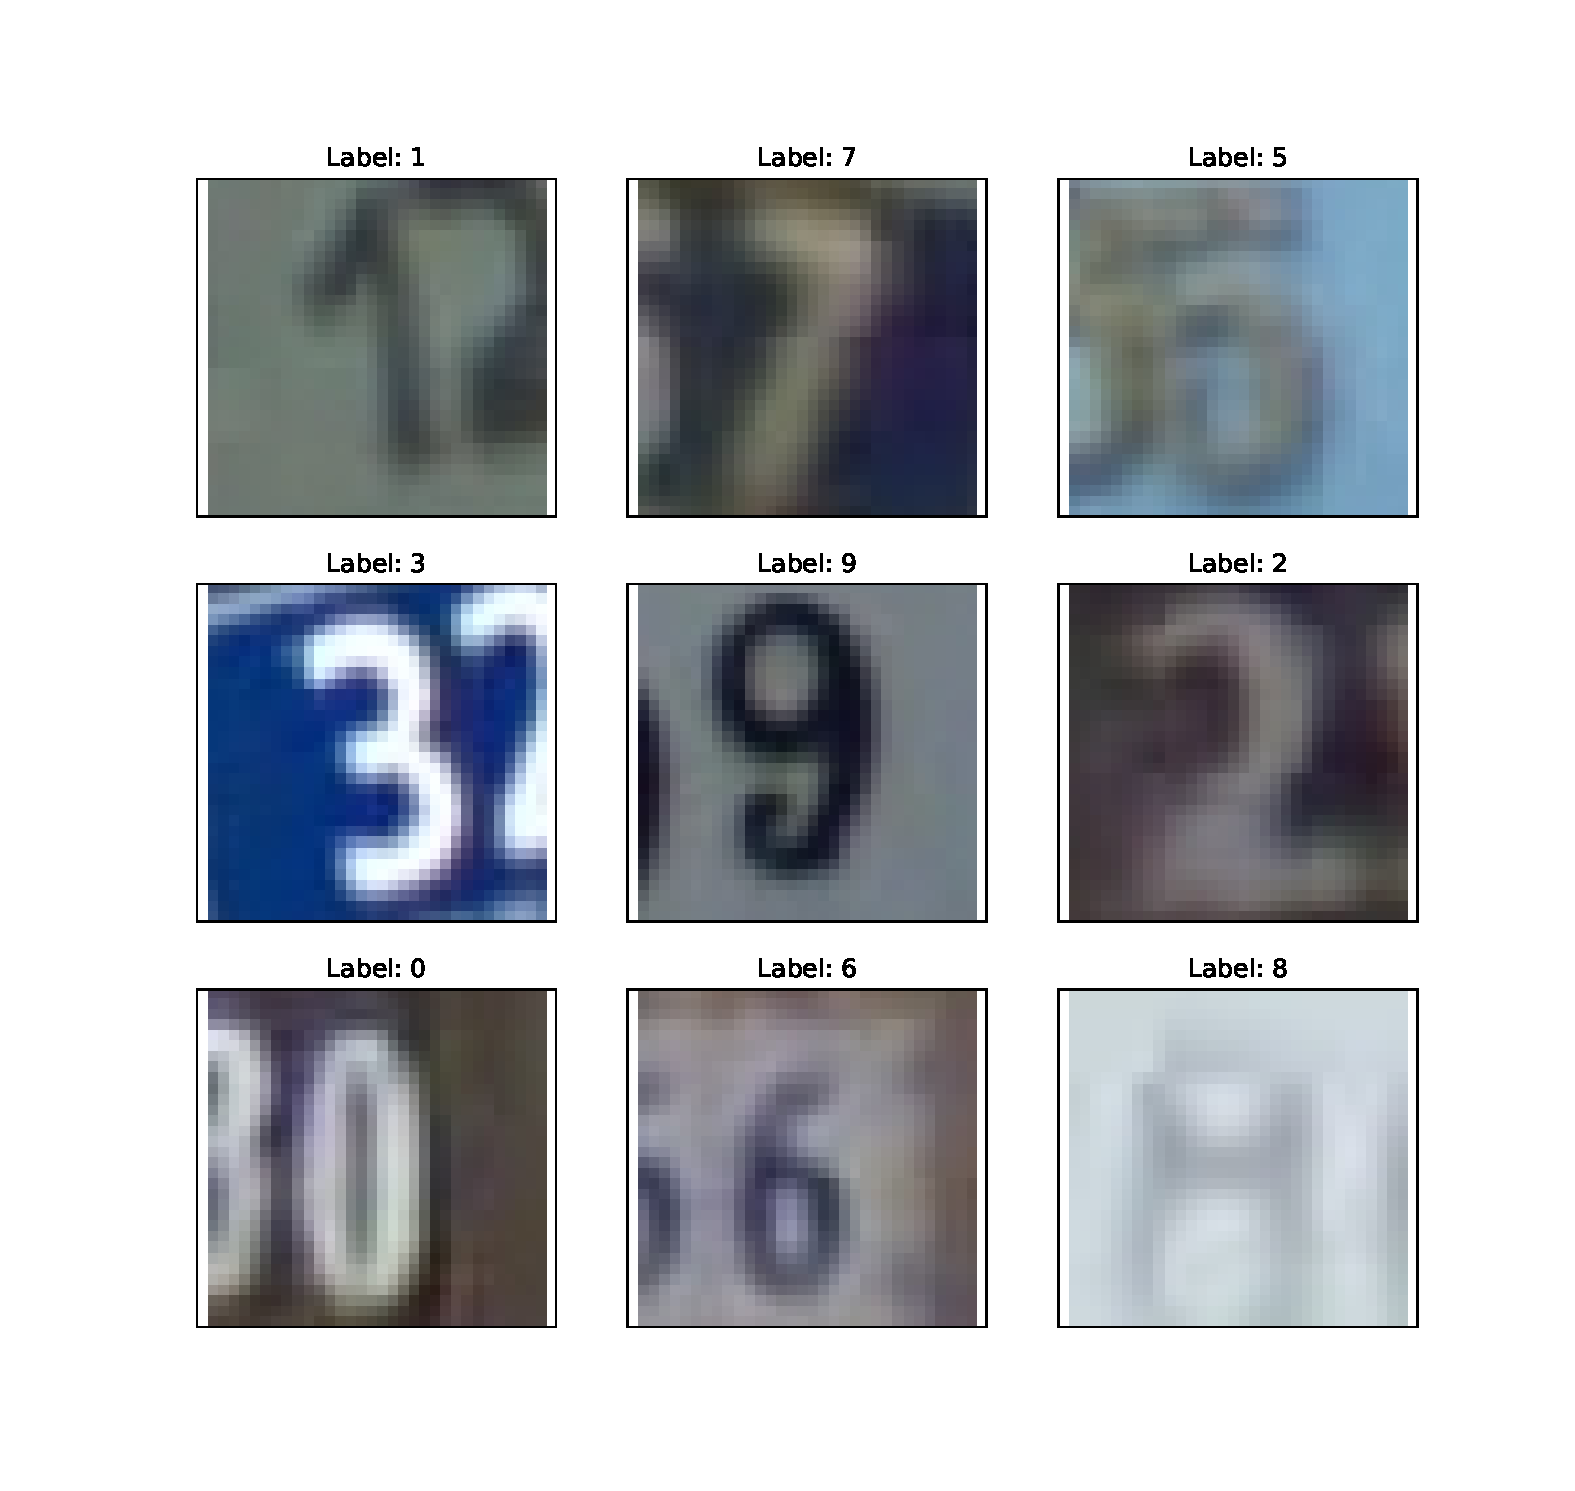
\includegraphics[width=0.8\textwidth]{Chapters/3.Implementation/figures/cSVHN.pdf}
    \caption[cSVHN example]{Nine images from the cSVHN dataset.}
    \label{fig:csvhn}
\end{figure}

The whole image set is split into three sets, a training set containing 73257 digits, a test set of 26032 digits, and a simplified \textit{"extra"} image set of 531131 images, claimed by the creator to be "less difficult." This extra, simplified image set is the one used in the experiments in chapter \ref{exp2} for task 3a, 3b, and 4 and both tasks in chapter \ref{exp3}.

\begin{table}[h]
    \centering
    \begin{tabular}{ccc}
    Class number (Digit) & Number of samples & \% of whole data set\\
    0                    & 45550             & 8.6\%               \\
    1                    & 90560             & 17.0\%              \\
    2                    & 74740             & 14.1\%              \\
    3                    & 60765             & 11.5\%              \\
    4                    & 50633             & 9.5\%               \\
    5                    & 53490             & 10.1\%              \\
    6                    & 41582             & 7.8\%               \\
    7                    & 43997             & 8.3\%               \\
    8                    & 35358             & 6.7\%               \\
    9                    & 34456             & 6.5\%              
    \end{tabular}
    \caption{Distribution of samples on each class in the cropped SVHN set used in this thesis, along with the portion of the whole set each class constitute. Given a random selection of samples from this set, this percentage should approximately be the probability of selection each class}
    \label{tab:SVHN}
\end{table} 

Because these images are from the real world, and because of the nature of house numbers, the class distribution is not even. In table \ref{tab:SVHN} the number of digits in each class in the extra set is listed along with the portion of the whole set this constitutes.  
